

\documentclass{article}
\usepackage{graphicx}
\usepackage{hyperref}
\usepackage{amsmath}
\usepackage{float}
\usepackage{subcaption}
\usepackage[margin=1in]{geometry} % Adjust the margins for better fit
\newcommand{\mycomment}[1]{}
\title{Automated Laundry Sorting Using Neural Networks}
\author{Dominik Krawiec s16941, Mateusz Darnowski s18322}
\date{}

\begin{document}

\maketitle
\newpage

\tableofcontents
\newpage



\section{Introduction}

\subsection{Background}
Categorizing clothes by color in preparation for washing to avoid color bleeding is one of the most ubiquitous mundane tasks around the house. It is not a complex task but is very time-consuming and highly subject to human error. Such routine tasks could be automated with the advancement of artificial intelligence and machine learning to high efficiency and great accuracy. This exercise involves the use of neural networks in performing laundry sorting. In doing so, it will sort them according to the 'dark', 'white', and 'colored' categories of their colors. More interestingly, this process makes this approach take a close dimension to some of the cognitive processes in the human brain associated with issues of pattern recognition and consequent decision-making, hence opening avenues for overlap between technological and neuroscience domains.
\subsection{Objective}
The focus of this project is the development of an efficient and correct neural network model that separation of the colors into 'dark', 'white', and 'colored' from which will then be fine-tuned with real-time user inputs for better performance. This fine-tuning done by humans is of prime importance in allowing the model to pick up specific nuances in color classification that it did not capture earlier from training on synthetic dataset. Lastly, this will be displayed through a graphical user interface showing real-time sorting by the model. The project has also given insight into how AI would simulate processes in the human brain, like learning, adaptation, and recognition of patterns, through computational simulation of cognitive functions.
\subsection{Scope}
Scope This project is divided into various phases, which shape a comprehensive scope touching on all the most important neural network development and implementation tasks. These are:
\begin{itemize}
    \item \textbf{Data Generation:} Generates synthetic data of very vast colors. This base color will be categorized with regard to its brightness, making the dataset very strong for initial model training.
    \item \textbf{Model Training:} The synthetic dataset will be used in training a neural network. This step will involve the division of the dataset into a training dataset, validation dataset, and test dataset, standardizing the features of a model and optimizing its hyperparameters to attain optimal performance of the model.
    \item \textbf{Fine-Tuning:}  After initial training, the model is fine-tuned by user input, which corrects and refines the model's predictions. A custom-developed GUI is provided to users to classify the colors shown on the screen to implement this purpose. Fine-tuning occurs in much the same way as humans learn—by making decisions based on experience and feedback, then gradually improving those decisions over time.
    \item \textbf{Model Comparison:} The performance of the initial and fine-tuned models is evaluated and compared using various graphical analyses, including confusion matrices, t-SNE, PCA visualizations, and 3D scatter plots. This comparison highlights the improvements achieved through fine-tuning and showcases the model's enhanced ability to recognize and categorize colors accurately.
    \item \textbf{Graphical User Interface Implementation:} A real-time GUI will be developed which showcases the capability of the model in sorting. This provides interactivity and visualization of the predictions made by the model about the laundry items for sorting, simulating actual sorting. The GUI does not only act as practical advice but also enhances the user's engagement because of the visualization, similar to the way a brain processes through vision.
  \end{itemize}

This structured approach ensures a thorough development and evaluation of the neural network, highlighting the importance of user feedback in enhancing machine learning models. By drawing parallels to human cognitive functions, this project not only demonstrates the potential of AI in automating household tasks but also offers a glimpse into how artificial systems can emulate complex brain processes. The graphical analyses provide deep insights into the model's performance, while the interactive GUI showcases its practical applications in a household setting.
\begin{itemize}
    \item \textbf{Data Generation:} Synthetic data representing a wide range of colors are generated. Each color is categorized based on its brightness, providing a robust dataset for initial model training.
    \item \textbf{Model Training:} The synthetic dataset is utilized to train the neural network. This involves splitting the data into training, validation, and test sets, followed by standardizing the features and optimizing the model's hyperparameters to achieve optimal performance.
    \item \textbf{Fine-Tuning:} Post initial training, the model undergoes a fine-tuning process where user input is employed to correct and refine the model's predictions. This phase is facilitated by a custom-developed GUI that allows users to classify colors displayed on the screen.
    \item \textbf{Model Comparison:} The performance of the initial and fine-tuned models is evaluated and compared using various graphical analyses, including confusion matrices, t-SNE, PCA visualizations, and 3D scatter plots. This comparison highlights the improvements achieved through fine-tuning.
    \item \textbf{Graphical User Interface Implementation:} A real-time GUI is developed to demonstrate the model's sorting capabilities. This interface provides an interactive and visual representation of the model's predictions, simulating the actual sorting of laundry items.
\end{itemize}

\section{Data Generation}
\subsection{Description}
Synthetic data of colors were generated, each of which belonged to one of the three classes based on its brightness. This will ensure that the model learns from examples that are different enough, covering the whole RGB color space.
\subsection{Color Categorization}
The brightness of each color is calculated using the formula:
\[ \text{brightness} = 0.299 \cdot R + 0.587 \cdot G + 0.114 \cdot B \]
Based on the brightness value, colors are categorized into three classes:
\begin{itemize}
    \item \textbf{Dark}: brightness < 85
    \item \textbf{White}: brightness > 170
    \item \textbf{Colored}: 85 $\leq$ brightness $\leq$ 170
\end{itemize}
This categorization helps in simulating the human decision-making process when sorting laundry.

\newpage

\subsection{Visualization}
A scatter plot was created to help visualize the distribution of the generated synthetic data, showing the RGB. Values of the colors and their respective categories. This plot is very useful in learning the initial dataset diversity and how well it covers the color spectrum.
\begin{figure}[H]
    \centering
    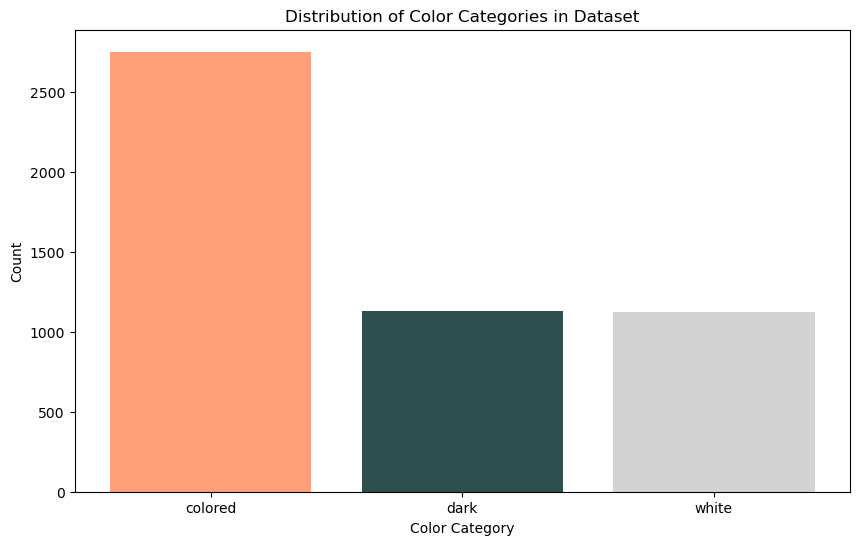
\includegraphics[width=\textwidth]{pictures/dis_out.png}
    \caption{Distribution of Generated Data}
    \label{fig:dis_out}
\end{figure}

Figure \ref{fig:dis_out} is a bar chart showing the distribution of colors over the three categories: dark, white, and colored. Each bar is colored to match the category it represents: colored in peach, dark in dark green, and white in light gray. This synthetic data is used for training the neural network. During the training process, it is determined whether the model can effectively learn the difference between colors.

\newpage

\section{Model Training}

\subsection{Dataset Preparation}
This synthetic dataset that was generated earlier was instrumental in training the neural network. The dataset contained a variety of colors, all labeled against one of the three classes: dark, white, and colored. Therefore, in order to make this model perform well on unknown data, this dataset is split into three parts: a training set, a validation set, and a test set. The model was trained using the training set, tuned using the validation set, and ultimately evaluated for performance on the test set.

These were then standardized by a Standard Scaler, which is important in neural networks since all features have to contribute equally towards learning. Standardization adjusts the scale of features so that the mean is zero and the standard deviation is one. This step is very critical to ensure that the model will be able to learn from the data efficiently.

\subsection{Model Architecture}
The neural network model was designed to be both simple and effective for the task of color classification. The architecture consisted of the following layers:

\begin{itemize}
    \item \textbf{Input Layer:} This layer had 3 units, one for each of the RGB color components.
    \item \textbf{Hidden Layers:} The model has two hidden layers, with each of them using the ReLU—Rectified Linear Unit—activation functions. ReLU is one of the activation functions applied in most cases to help the model learn complex patterns.
    \item \textbf{Output Layer:} The output layer had 3 units with a softmax activation function. The softmax function converts the output into a probability distribution, making it suitable for multi-class classification. Each unit in this layer corresponds to one of the three color categories (dark, white, colored).
\end{itemize}

This architecture was chosen in view of the requirement for striking a balance between model complexity and computational efficiency. The hidden layers give this model a chance to understand intricate patterns in color data, while an output layer provides equal classification capability.
\subsection{Hyperparameter Tuning}

The most important stage in the development of a high-performing neural network is hyperparameter tuning, which includes finding the combination of hyperparameters that provide maximum performance. In this project, Keras Tuner has been used along with the Hyperband algorithm. In other words, this algorithm enables very wide searches of the space for hyperparameters by genuinely distributing resources dynamically across promising configurations.
The hyperparameters tuned in this process included:
\begin{itemize}
    \item \textbf{Number of Units in Hidden Layers:} The search space ranging from 8 to 64 units per layer with an increment of 8.
    \item \textbf{Learning Rate:} This was to be done so that the optimal speed for which the model learns could be found.
    \item \textbf{Batch Size:} Various batch size were tested to find an optimal batch size for model.   \end{itemize}

With an exhaustive tuning process, the rest of the optimal hyper-parameters could be identified, thus ending up with a model configuration which gives maximum validation accuracy.
\subsection{Training Process}

The training process was done over 20 epochs, with early stopping implemented to prevent overfitting. Early stopping monitors validation loss and stops training if the validation loss doesn't improve for a certain number of epochs. This will guarantee generalization on new data, rather than the model memorizing training data.
During training, the model's performance was followed continuously with training and validation sets. The best model based on validation loss was kept for further evaluation. Training history is provided in Figure \ref{fig:accuracy_graph}, indicating accuracy and validation accuracy as a function of epochs.

\begin{figure}[H]
    \centering
    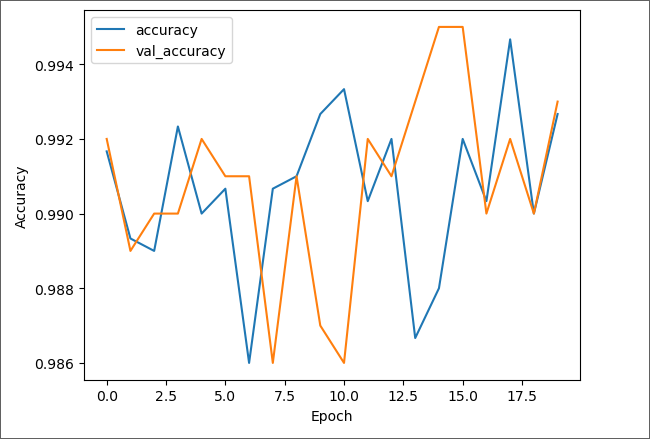
\includegraphics[width=\textwidth]{pictures/graph_1_training.png}
    \caption{Training and Validation Accuracy}
    \label{fig:accuracy_graph}
\end{figure}

The graph shows the model's learning curve, with fluctuations indicating the learning process's complexity and the model's ability to generalize from the training data to the validation data.

\subsection{Results}
After training, the best model was evaluated on the test set — essentially, data it had never seen. This is important because it gives the correct measure, unbiased performance of models under real-world scenarios.

Moreover, high test accuracy was achieved. This speaks to the generalization ability of the model from the training data to new unseen data. Again, this accuracy result stresses the effectiveness of the model architecture and the training process used in this research. This also underlines what tuning of hyperparameters and early stopping bring about in coming up with a robust machine learning model.

Generally, the training of the model was both systematic and thorough. For that, a neural network will be trained for the characterized classification of colors into dark, white, and colored. This forms a very solid base for the fine-tuning and practical application of the later stages of this project.\newpage


\section{Fine-Tuning with User Input}

\subsection{User Interface}
A GUI was developed to fine-tune the process. The users can classify colors displayed in the image into one of the categories defined, i.e., 'dark,' 'white,' or 'colored.' It is an iterative approach guided by user input with an active learning process, which means that the model progressively enhances accuracy in real-time due to the interactive nature of the GUI.

\begin{figure}[H]
\centering
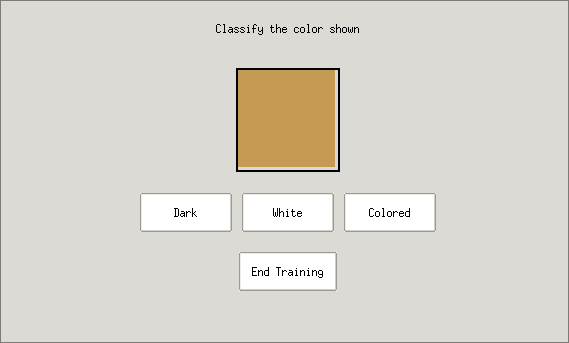
\includegraphics[width=\textwidth]{pictures/user_fine_tuning_GUI.png}
\caption{User Interface for Fine-Tuning}
\label{fig
}
\end{figure}

\subsection{Process Overview}
The fine-tuning process consisted of the following steps:

\begin{itemize}
\item \textbf{Display Colors:} The GUI displays a color to the user, who is then requested to classify it by clicking one of the buttons named 'Dark', 'White', or 'Colored'. This teaches the model and allows its predictions to be adapted based on user input.
\item \textbf{Model Update:} The model weights are updated after each classification; this is done by fitting the model on the newly labeled data point and incrementally improving performance over time.
\item \textbf{Saving the Fine-Tuned Model:} Once enough colors have been classified by fine-tuning from the user's actions, the fine-tuned model is saved. This model contains user modifications and refinements.
\end{itemize}

\subsection{Model Testing Results}
The fine-tuned model is subjected to tests to check how much the users' influence controls the performance of a model. While the base classification was performed with the help of some default algorithm, the fine-tuned model represents a rather humanized way of color classification. Improvements brought by this process are reflected in the refined alignment with user-defined classifications.
\newpage

\section{Model Comparison}
\subsection{Evaluation Metrics}
The initial model and the fine-tuned model were compared using confusion matrices to visualize how the fine-tuning process altered the model's understanding of colors. Additionally, dimensionality reduction techniques (t-SNE and PCA) were used to visualize the model predictions and assess the impact of fine-tuning.

\subsection{Confusion Matrix}
The confusion matrix in Figure \ref{fig:confusion_matrix} compares the predictions of the best model with the fine-tuned model. The rows represent the actual classes, while the columns represent the predicted classes. The diagonal elements show the number of correct predictions, while the off-diagonal elements indicate misclassifications.

\begin{figure}[H]
    \centering
    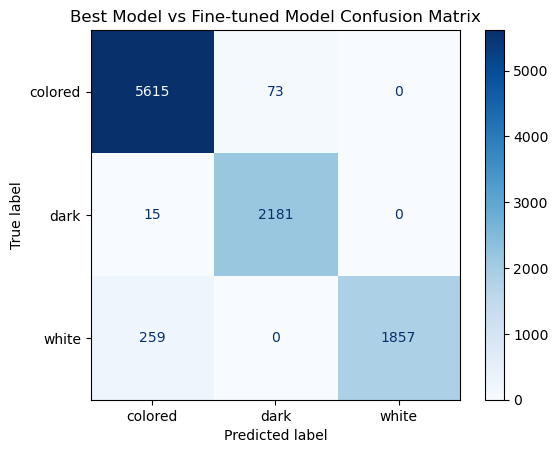
\includegraphics[width=\textwidth]{pictures/graph_1_comp.png}
    \caption{Best Model vs Fine-tuned Model Confusion Matrix}
    \label{fig:confusion_matrix}
\end{figure}

The confusion matrix helps visualize how the fine-tuning process has altered the model's understanding of colors. Each entry in the matrix shows the number of instances where the best model's prediction (true label) matches or differs from the fine-tuned model's prediction (predicted label). By examining the off-diagonal entries, we can see where the two models disagree, highlighting the changes introduced by fine-tuning.

\subsection{Dimensionality Reduction Analysis}
Dimensionality reduction techniques, t-SNE and PCA, were used to visualize the distribution of the model's predictions. Figures \ref{fig:tsne_pca_best} and \ref{fig:tsne_pca_fine_tuned} illustrate the results for the best model and the fine-tuned model.

\begin{figure}[H]
    \centering
    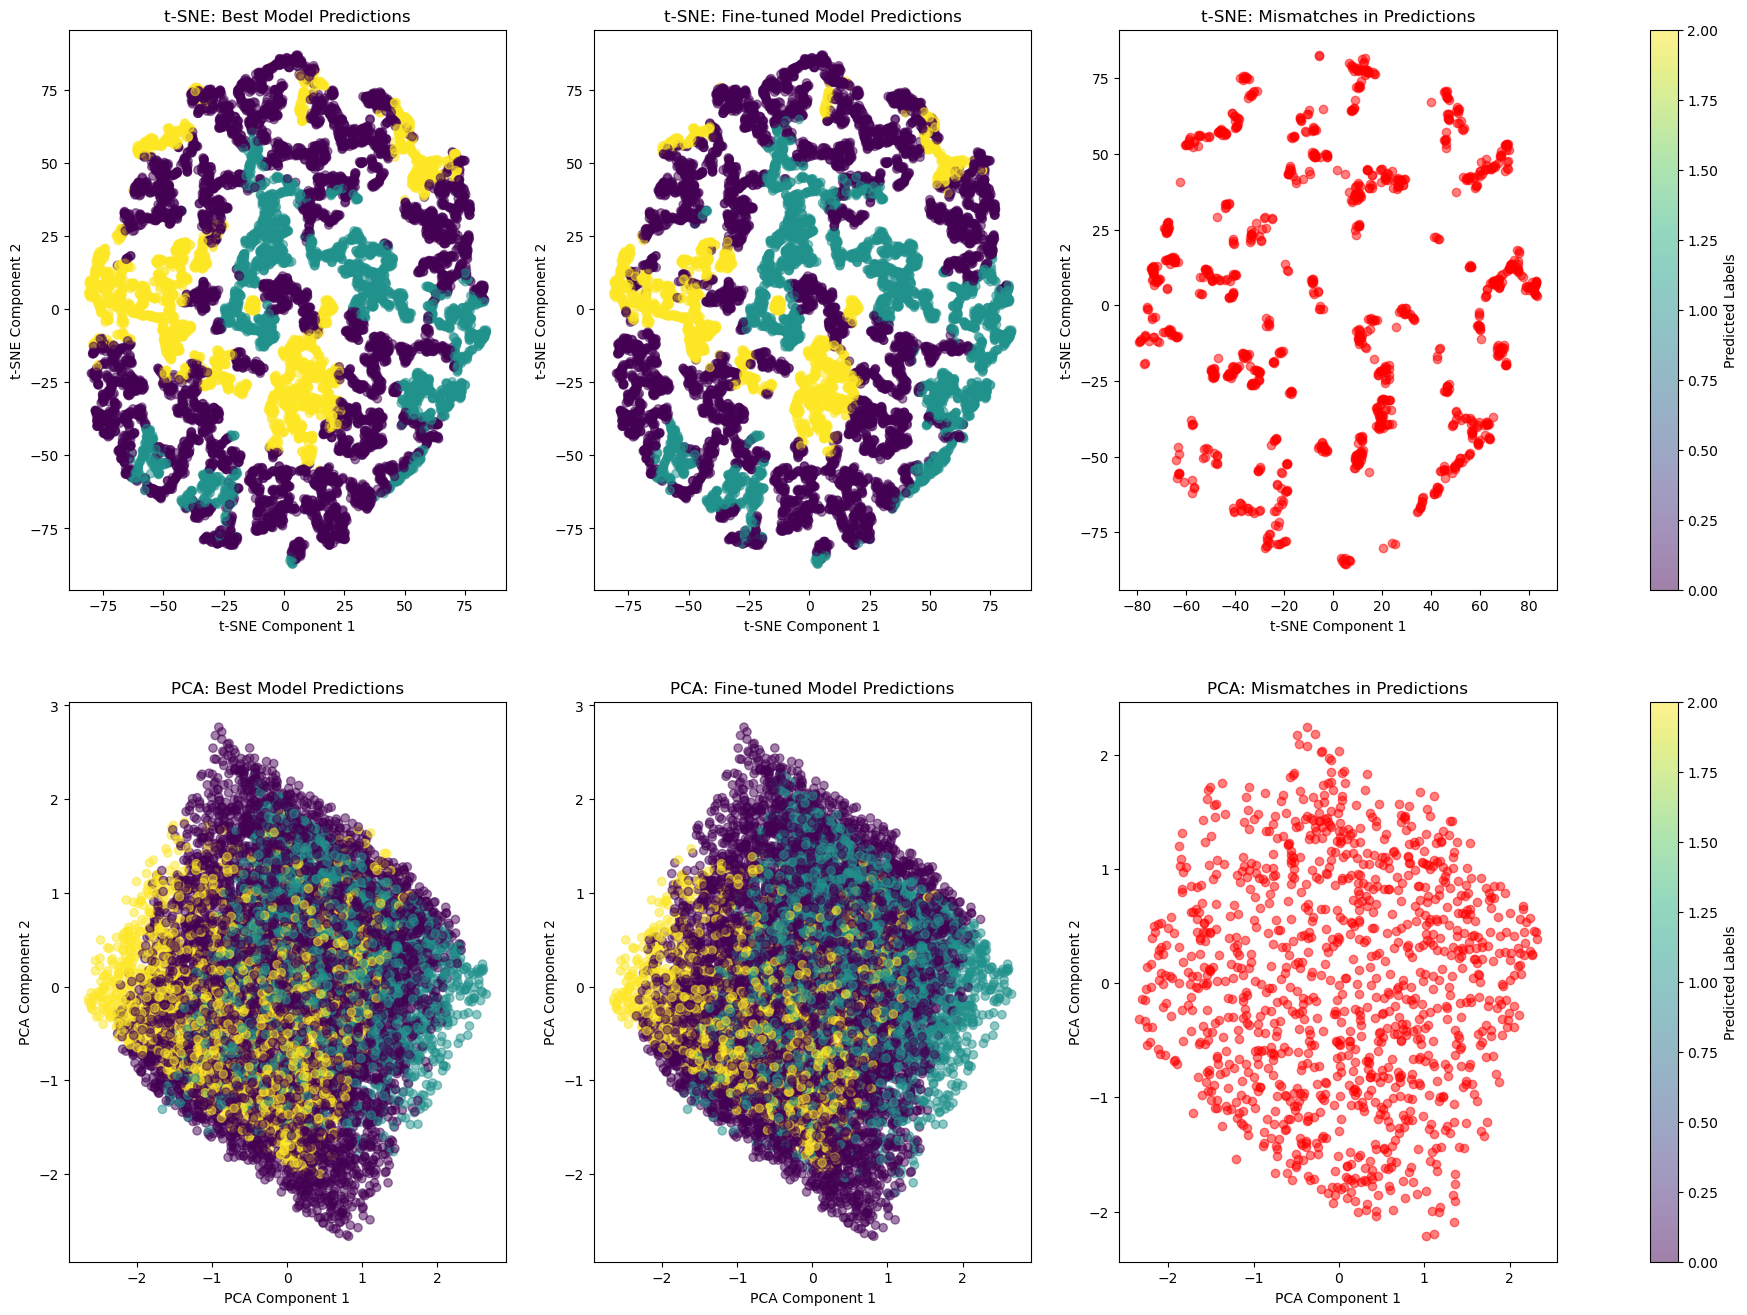
\includegraphics[width=\textwidth]{pictures/graph_2_comp.png}
    \caption{t-SNE and PCA Visualizations for Best Model Predictions}
    \label{fig:tsne_pca_best}
\end{figure}

\begin{figure}[H]
    \centering
    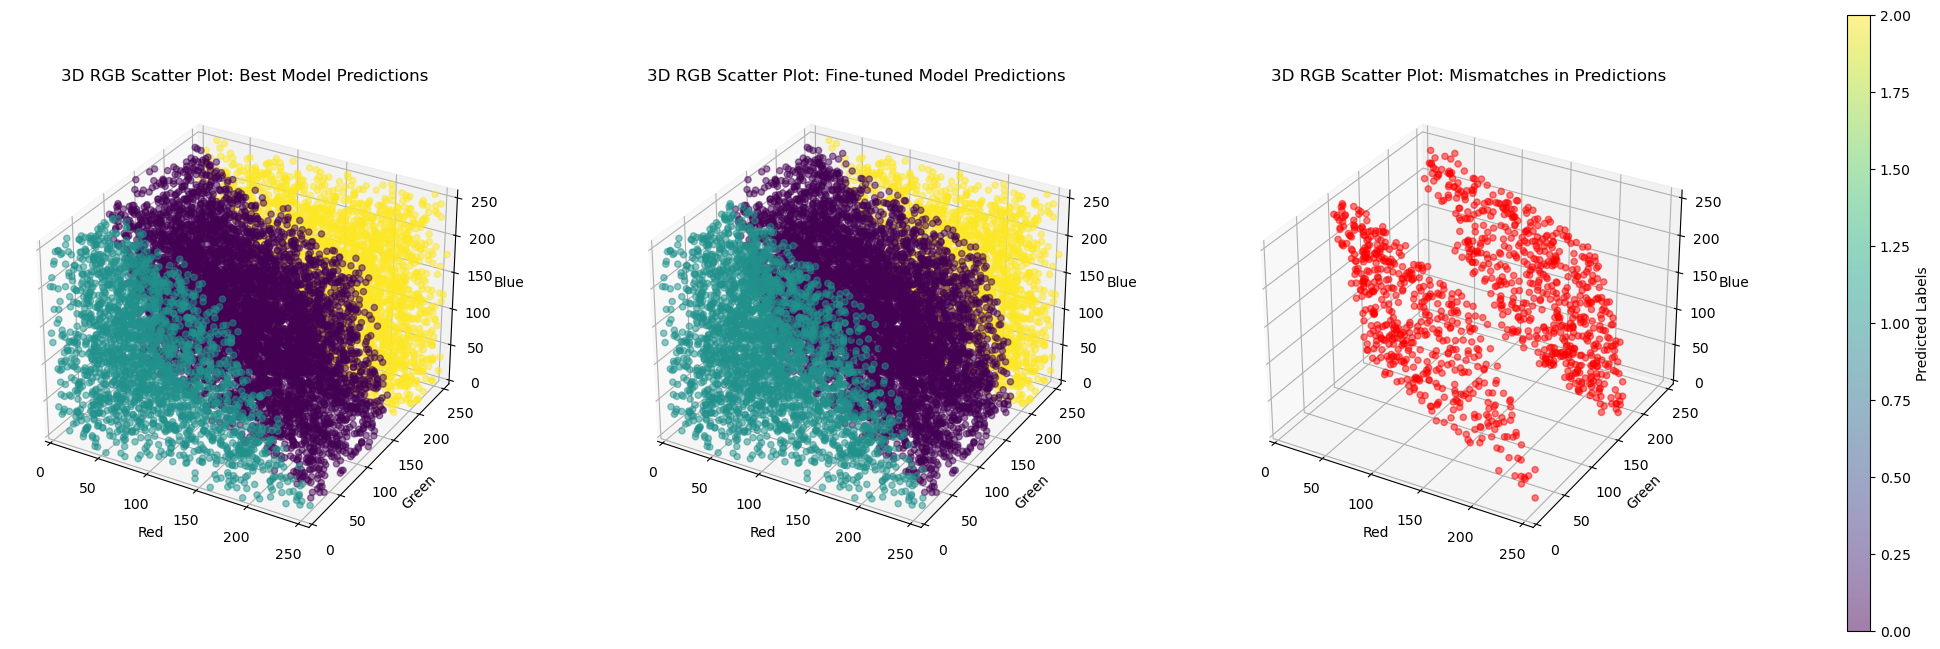
\includegraphics[width=\textwidth]{pictures/graph_3_comp.png}
    \caption{t-SNE and PCA Visualizations for Fine-Tuned Model Predictions}
    \label{fig:tsne_pca_fine_tuned}
\end{figure}

The differences between the color categories in both t-SNE and PCA visualizations are represented by the clusters of the models. The fine-tuned model displays somewhat more defined clusters, thus indicating better separability of the three color categories. This would mean that the fine-tuning process has allowed the model to pick up very subtle differences in color classification so the prediction can be better aligned with human judgment. The more apparent visual separation in the fine-tuned model indicates a higher understanding of the color space, leading to more nuanced classification.

\subsection{Mismatch Analysis}
The mismatch analysis in Figure \ref{fig:mismatch_analysis} highlights the discrepancies between the predictions of the best model and the fine-tuned model. The visualizations show the mismatches in a 3D RGB space, PCA space, and t-SNE space.

\begin{figure}[H]
  \centering
    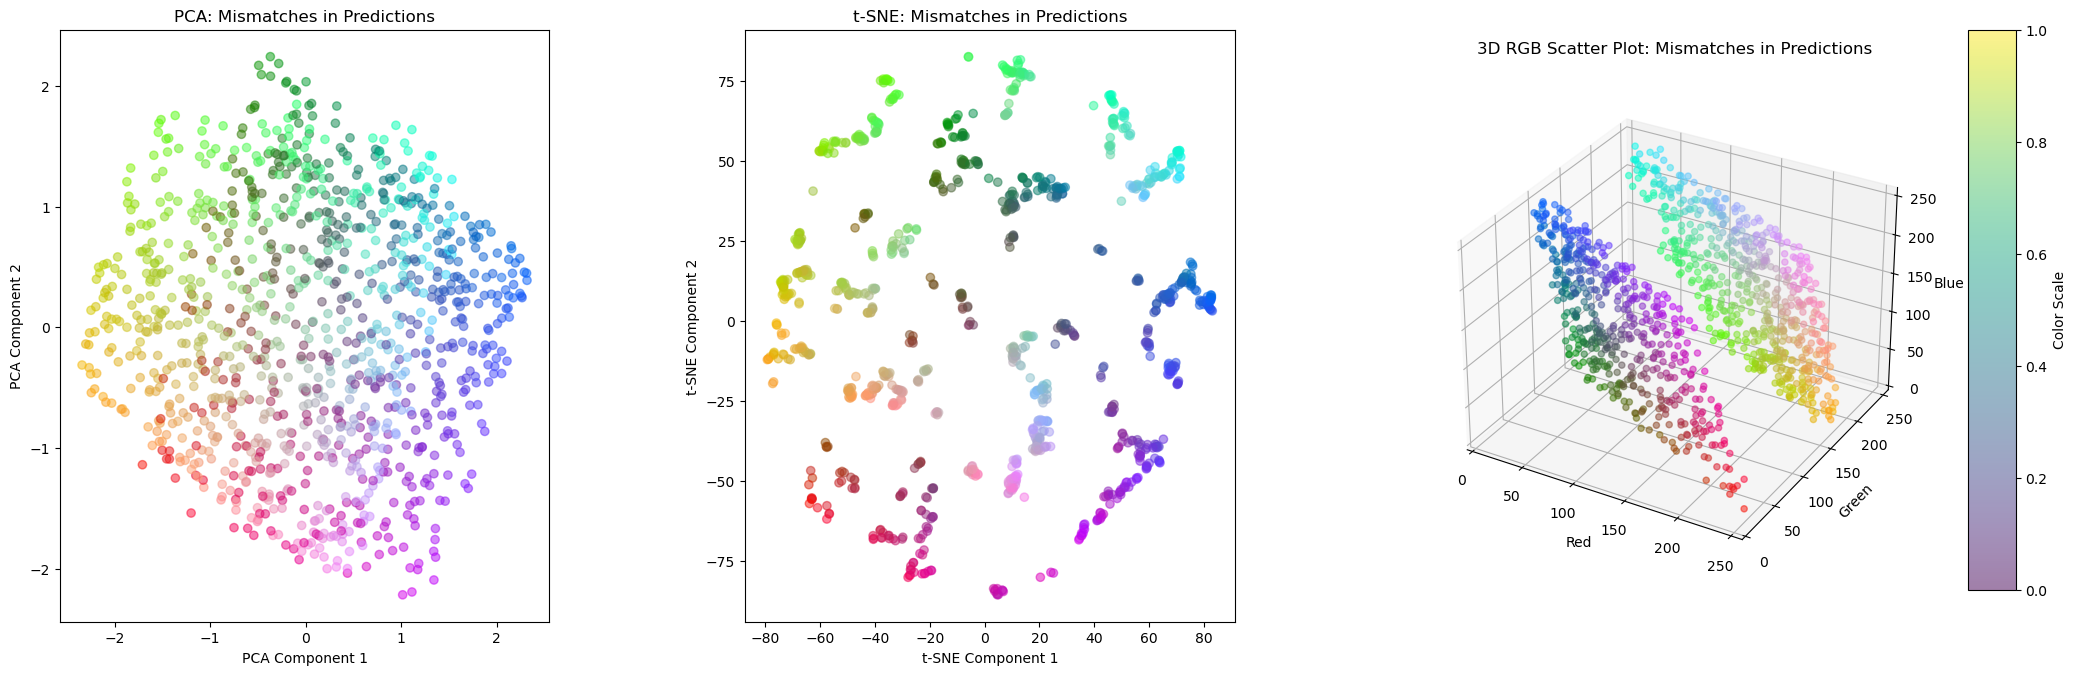
\includegraphics[width=\textwidth]{pictures/graph_4_comp.png}
    \caption{Mismatch Analysis}
    \label{fig:mismatch_analysis}
\end{figure}

The mismatch analysis reveals areas where the best model's predictions differed from those of the fine-tuned model. In the 3D RGB scatter plot, the mismatched points are highlighted, showing specific regions in the color spectrum where the fine-tuned model diverges from the best model. This divergence is also evident in the PCA and t-SNE visualizations, where the points indicating mismatches are dispersed differently for each model.

The fine-tuning process readjusts model predictions to be closer to what is suggested by the user who fine-tunes the network. This could especially be valuable in scenarios where human-like accuracy and intuition are of importance.

In essence, it is clear from the graphical analyses that both models are of very high accuracy, but the fine-tuned model has a user-centered way of capturing nuances, which makes it applicable in practical applications such as the sorting of laundry.
\newpage


\section{Real-Time Simulation of Laundry Sorting}
\subsection{GUI Design and Implementation}
Laundry is sorted in real time using a GUI for categorization purposes, and a neural network is then used to sort the laundry according to color. This interface provides an interactive way to interact with a model's real-world application through visual means.
\subsection{GUI Features}
The GUI offers following features:
\begin{itemize}
\item \textbf{Model Loading:} Preprocessing tools needed for color classification based on a scalar and a label encoder are loaded along with a trained neural network model.
\item \textbf{Real-Time Color Prediction:} The GUI displays random items colored and predict by category. It is either 'dark', 'white', or 'colored' by use of our model.
\item \textbf{Sorting Animation:} It animates the items to fall into the right laundry bags based on what the model has predicted. The sorting process is animated, making it easily traceable by the user at a glance.

\item \textbf{Counters:} The GUI maintains counters for each bag and increments them in real-time as items are sorted to them. Through counters, the user is informed of the number of items that have been classified into a particular category.
\end{itemize}

\begin{figure}[H]
\centering
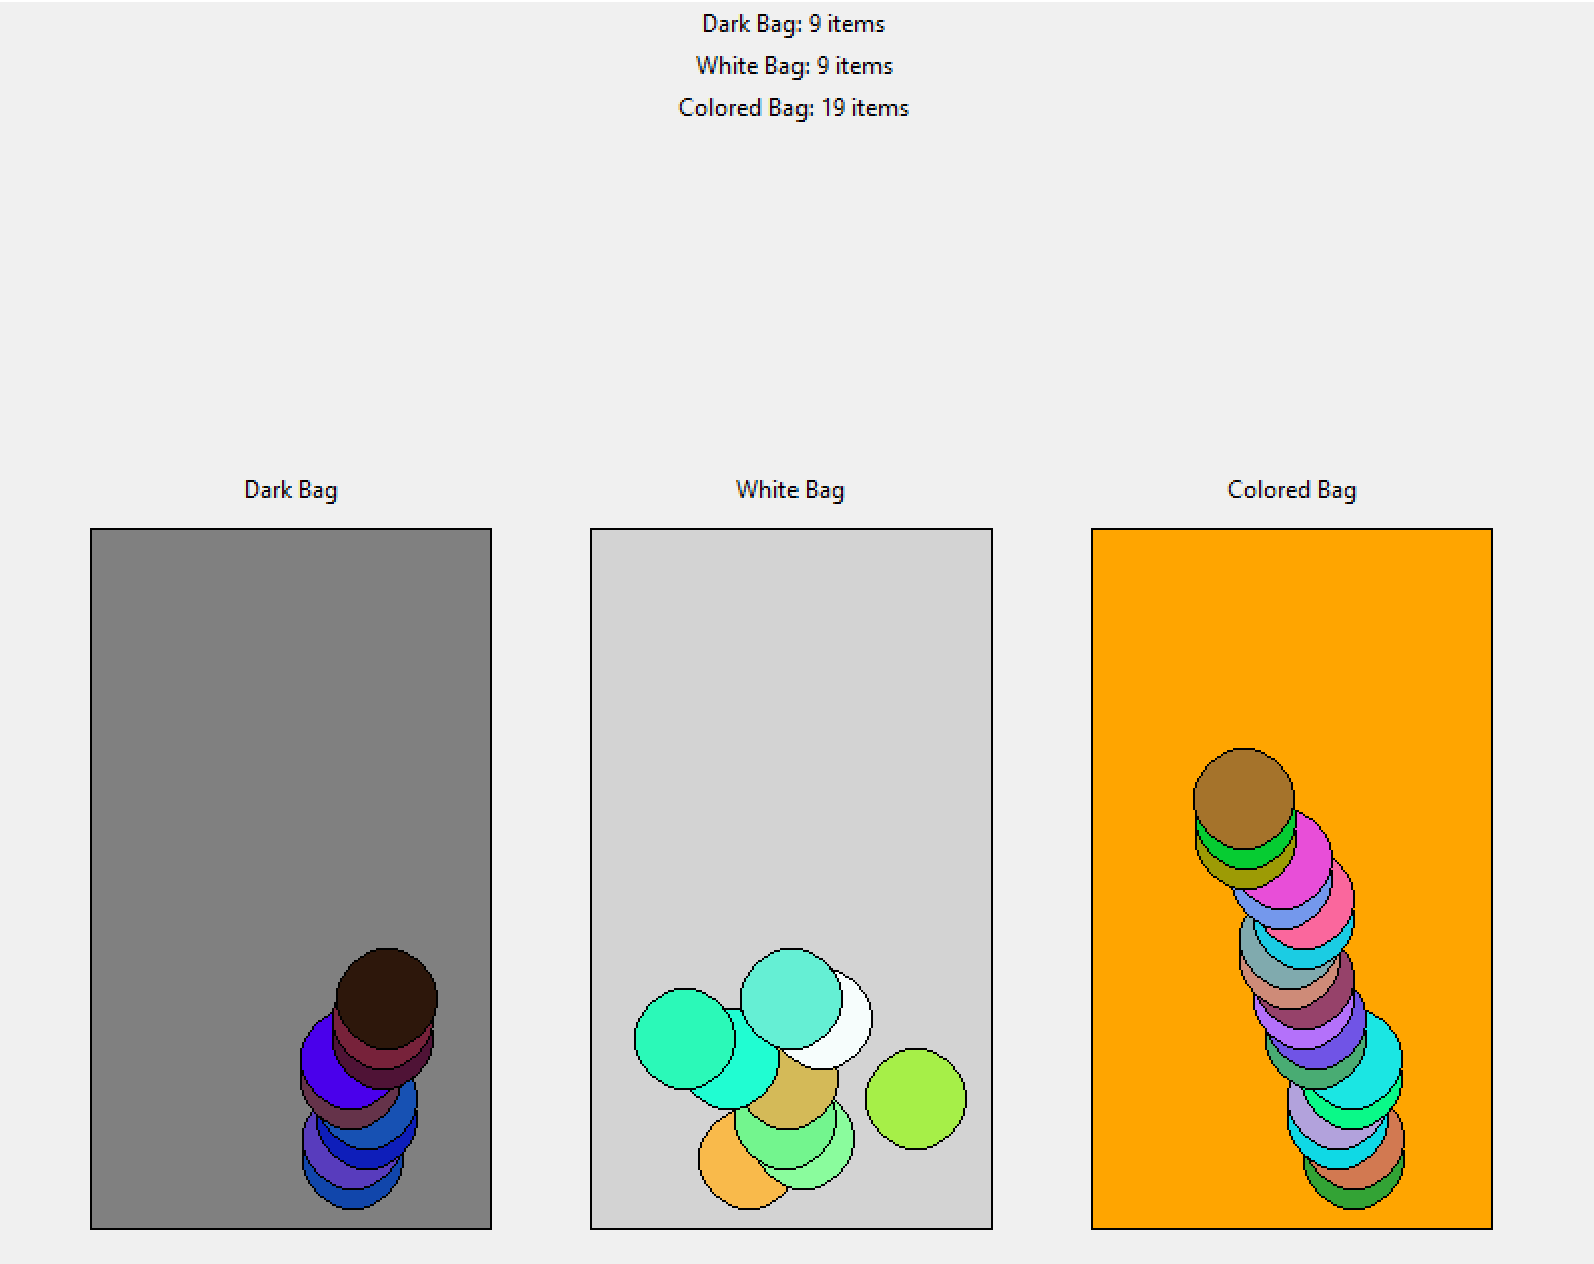
\includegraphics[width=0.8\textwidth]{pictures/gui_example.png}
\caption{Graphical User Interface for Real-Time Sorting Simulation}
\label{fig
}
\end{figure}
\newpage

\section{Human Brain References}

\subsection{Pattern Recognition}
The neural network color-sorting ability may be indirectly viewed as working like the human brain, which functions on principle-based pattern recognition. Any information that is visual is analyzed by the human brain visual cortex in a manner that involves detection and interpretation of patterns by interpreting light and color. Similarly, neural networks process input data through different layers to fit the patterns for decision-making. For example, edges are identified by the visual cortex, and textures. These are comparable to the ways in which neural networks would extract features from input data.
\subsection{Learning and Adaptation}
In some respects, fine-tuning in neural networks may be seen to be like humans who learn and make corrections based on feedback. Humans are learning continuously from the responses thrown by the environment on their situated activities and adjusting their actions accordingly. This experiential learning is called. Basically, it is fine-tuning in neural networks with input from users, which refines its prediction with constant feedback just like humans do by learning from their mistakes and trying again. This iterative learning process enhances accuracy and adaptability of the model, similar to how synaptic connections between neurons are strengthened or weakened based on experience within the brain.
\subsection{Visual Processing}
The model treats information about color in a way it would be processed humanually. A human brain defines the nature of a color by its brightness and chromatic components, which are ranked in the visual cortex. Neural networks achieve this thing by representing colors numerically, for instance, using the RGB values, and then ranking them with the patterns learned. In the present project, using brightness to rank colors is similar to the way in which a brain makes use of luminance to tell apart the various types of visual stimuli. The GUI further emulates the real-time processing and decision-making capabilities of the brain, thereby demonstrating how AI is able to emulate human cognitive capabilities in applications that are relevant to real life.
\subsection{Graphical Analysis of Results}
The plots present studies of the base and fine-tuned models' color classification accuracy. Both models are highly accurate, as indicated by the confusion matrix, with the latter a little bias towards more human-like classifications. According to t-SNE and PCA visualization, distinct clustering of color categories for the cases can be noted, with more defined clusters shown by the fine-tuned model that demonstrates better differentiation and understanding of the color space. Off-note analysis underlines the discrepancies between the predictions of the initial model and those of the fine-tuned model, showing the improvements added by the incorporation of user feedback. The effect of such analyses aligns very well with the capacity of the brain to adapt and fine-tune its cognitive processes based on experience and feedback, underscoring similarities between neural network training and human learning.

The findings convey the face that neural networks learn performance and how to improve on that performance through feedback and adaptation, similar to the human brain. This approach could teach AI in complex, cognitive processes found in everyday applications, such as automated laundry sorting.

\newpage

\section{Conclusion}

\subsection{Summary}
The project successfully developed a neural network model for sorting laundry colors. The process involves creating a synthetic data collection, training, fine-tuning with user feedback, and evaluating overall performance. The model was first trained on a very wide variety of synthetic colors and showed high accuracy in categorizing colors into dark, white, and colored classes. This model was further fine-tuned based on user input to go more in line with human perception and classification.
\subsection{Future Work}
Future improvements could include:
\begin{itemize}
  \item \textbf{Incorporating Real-world Data:} Although synthetic data offers a strong basis, utilizing real-world data might enhance the models' suitability and resilience for practical uses.
  \item \textbf{Advanced Feedback Mechanisms:} To further refine the model, more complex user feedback methods can be implemented. This may also involve continuous learning, in which models are continuously updated by users to make improvements in real time.
  \item \textbf{Exploring Additional Features:}  In addition to brightness and fundamental color components, other variables that can be utilized for even better classifiability include texture or material type.
 \end{itemize}
\subsection{Applications}
The methodology and the approach followed for this project have far-reaching applications beyond laundry sorting. Similar models can be worked out for a variety of categorization tasks within an industrial setting, including sorting by color or type in manufacturing lines, image recognition systems in quality control, and automation processes where the question of accurate classification arises. Integration of neural networks with user feedback mechanisms is considered a very powerful tool for making any system adaptive and intelligent, working like human cognition, therefore increase in efficiency and reduction of errors in day-to-day tasks.
\end{document}